\centerline{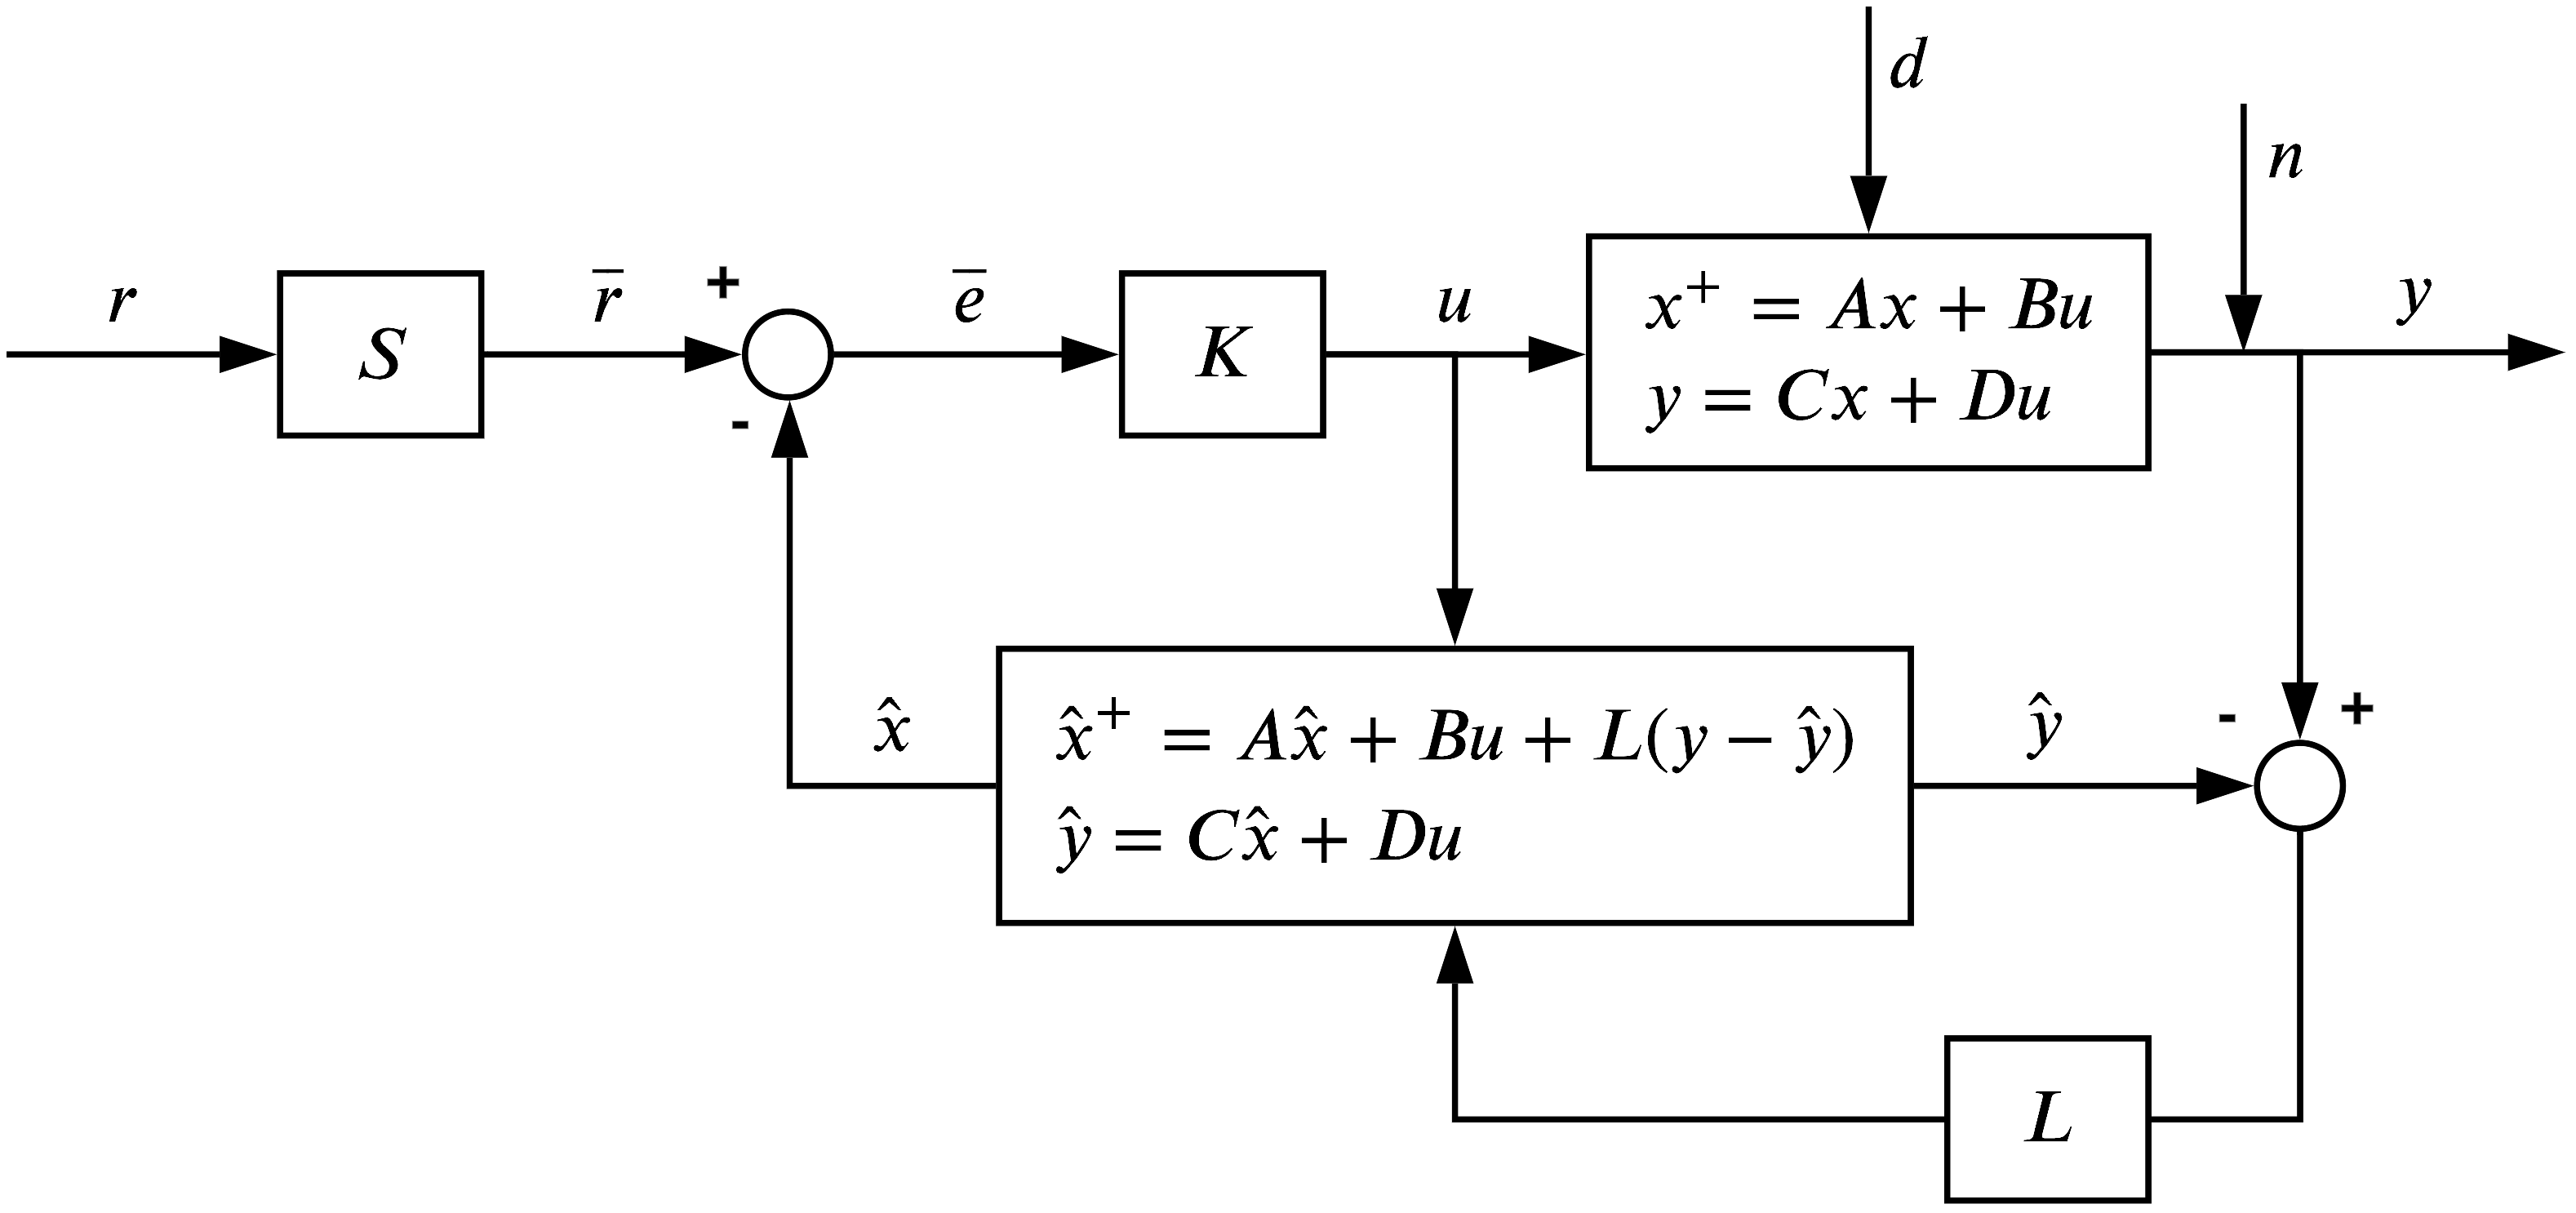
\includegraphics[width=1\linewidth]{src/5_dynamic_output_feedback/images/dofb.png}}

\subsection{LQG}
\begin{align*}
    \begin{bmatrix}
        x \\
        \eta
    \end{bmatrix}^+
    &= \begin{bmatrix}
        A - BK & BK \\
        0 & A - LC
    \end{bmatrix}
    \begin{bmatrix}
        x \\
        \eta
    \end{bmatrix} +
    \begin{bmatrix}
        BKS\\
        0
    \end{bmatrix} r\\
    y &= \begin{bmatrix} C & 0 \end{bmatrix}
    \begin{bmatrix}
        x \\
        \eta
    \end{bmatrix}
\end{align*}

\subsubsection{LQG Servo}
\begin{align*}
    \begin{bmatrix}
        x \\
        x_I \\
        \eta
    \end{bmatrix}^+\!
    &=\! \begin{bmatrix}
        A - BK & -BK_I & BK \\
        -C & 0 & 0 \\
        0 & 0 & A - LC
    \end{bmatrix}\!
    \begin{bmatrix}
        x \\
        x_I \\
        \eta
    \end{bmatrix}\! + \!
    \begin{bmatrix}
        BKS \\
        I \\
        0
    \end{bmatrix}\! r\\
    y &= \begin{bmatrix} C & 0 & 0 \end{bmatrix}
    \begin{bmatrix}
        x \\
        x_I \\
        \eta
    \end{bmatrix}
\end{align*}

\subsubsection{LQG Stability}
LQG guarantees closed loop stability, but the margins can be arbitrarily small.